
\chapter{ Material Overrides }

Based on Razroo best practices, we have established the easiest way to get 
your app up and running, is to use material design within your Angular 
application. Generally, an organization will want to roll it's own theme into 
Angular Material. When that happens the developer will have to go ahead and 
customize the build for material design. Let's talk about how we can go ahead 
and do that. 

\section{Understanding Colors in Material}
First and foremost it is important to understand something called a color 
palette. I know some of you might be aware of what it is, but personally, I was
not aware. A color palette in the digital world, refers to the full range of 
colors that can be displayed on a device. Within a material design application 
it refers to the range of colors that can be used within the application. 
Material's design language makes use of two main colors for it's color palette: 

\subsection{Primary and Secondary Values}
\begin{enumerate}
  \item Primary - Color displayed most frequently across your app's screens and
  components. 
  \item Secondary - "Provides more ways to accent and distinguish your product."
  \begin{enumerate}
    \item Floating Action Button(Literally buttons that float over main content)
    \item Selection controls(sliders, switches etc.)
    \item Highlighting selected text
    \item Progress bars
    \item Links and headlines
  \end{enumerate}
\end{enumerate}

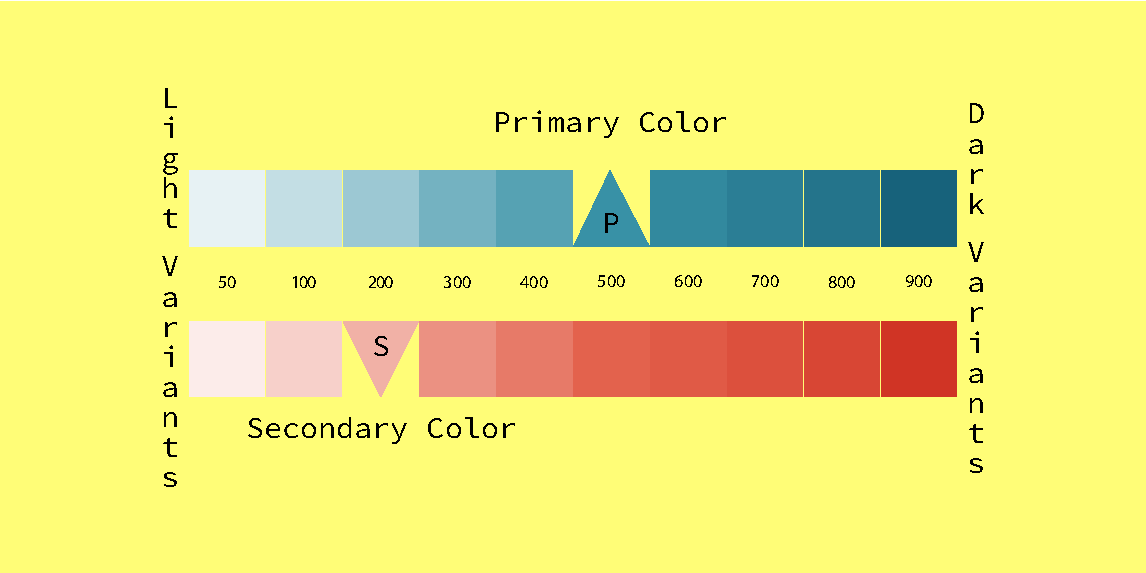
\includegraphics[width=414pt]{design-language-system/material-overrides/material-design-palette_pt.pdf}

\subsection{Material Color Maps}

It will then create a series of light and dark variants based on the primary 
and secondary values. The primary and second values must be a map of colors 
going from lightest(50) to darkest(900). 

Material has already created a series of 16 color maps, for it's design system. 
An example of material green color map, for instance, will look something like 
this: 
\begin{lstlisting}
$mat-green: (
  50: #e8f5e9,
  100: #c8e6c9,
  200: #a5d6a7,
  300: #81c784,
  400: #66bb6a,
  500: #4caf50,
  600: #43a047,
  700: #388e3c,
  800: #2e7d32,
  900: #1b5e20,
  A100: #b9f6ca,
  A200: #69f0ae,
  A400: #00e676,
  A700: #00c853,
  contrast: (
    50: $dark-primary-text,
    100: $dark-primary-text,
    200: $dark-primary-text,
    300: $dark-primary-text,
    400: $dark-primary-text,
    500: $dark-primary-text,
    600: $light-primary-text,
    700: $light-primary-text,
    800: $light-primary-text,
    900: $light-primary-text,
    A100: $dark-primary-text,
    A200: $dark-primary-text,
    A400: $dark-primary-text,
    A700: $dark-primary-text,
  )
);
\end{lstlisting}

For primary values, the regular value will start at 500. For secondary values, 
the regular value will start at 200. The significagance of these values is that 
Material Design will follow a Hierarchical system. The darker the color is, the 
more of an emphasis we are placing on that button. The lighter it is, the less 
emphasis we are placing on that element. 

\mybox{You might be wondering about two things. For starters, why it is that 
the values progress by 100's. Second what is up with the values that have an 
"A" attached to the left side. Values progress by 100's is merely a convention
used by Material Desing. Other design frameworks progress by 10's(IBM Design)
instead of 100's, for instance, or even by 1's(Open Color). It is merely a
convention used to show that values are progressing.}

\section{Material Design and Sass}
First and foremost, we have already established that we will be working within
a Sass environment. Material Design offers Sass out of the box, and makes it 
incredibly easy to customize your environment based on sass overrrides. 

\section{Npm Install Material Theme}
First and foremost, let's make sure that we have properly installed and Angular
Material in our Angular application. 
\begin{lstlisting}
npm install --save @angular/material @angular/cdk @angular/animations
\end{lstlisting}

You package.json will now include packages needed to use Angular Material 
within the application in general. In addition, the package
(\lstinline{@angular/material}) to make the Sass changes we so dearly need. 

\section{Import Material Design and Call Core Styles}
The next step, is for us to go ahead and import Material Design in our 
\lstinline{styles.scss} file. The \lstinline{styles.scss} file can be found
in the root Angular application \lstinline{src} folder.

\begin{lstlisting}[caption=styles.scss]
@import '~@angular/material/theming';
// always include only once per project
@include mat-core();
\end{lstlisting}

\mybox{You will notice that we are adding a tilda\lstinline{\~} next to the
node module folder, containing the sass file we need. This tell the sass that
file we would like to import is located inside of the \lstinline{node\_modules}
folder.}

What the above does is import the \lstinline{theming.scss} file that contains
all of the theming variables for material design. We are also calling the
\lstinline{mat-core()} function, which is a, \begin{quote}
\say{Mixin that renders all of the core styles that are not theme-dependent.}
\end{quote} \footnote{This quote can be found in the \lstinline{_theming.scss}
file}

\section{Material Light + Dark Theme}
Angular offers out of the box in the \lstinline{_theming.scss} file a light and
dark theme function. The function looks a follows: 
\begin{lstlisting}
@function mat-light-theme($primary, $accent, $warn: mat-palette($mat-red)) {
  @return (
    primary: $primary,
    accent: $accent,
    warn: $warn,
    is-dark: false,
    foreground: $mat-light-theme-foreground,
    background: $mat-light-theme-background,
  );
}  
\end{lstlisting}

It takes in two required parameters: 
\begin{enumerate}
  \item primary - Primary color
  \item accent - Accent color 
\end{enumerate}
and one optional parameter called warn, which by default will be red. Material 
will also by default specify warn as being red. 

So let's say we wanted to create a custom theme based on some of the values 
that Angular provides, we can do the following: 

\begin{lstlisting}
$px-app-primary: mat-palette($mat-green);
$px-app-accent: mat-palette($mat-yellow);

$px-theme: mat-light-theme($px-app-primary, $px-app-accent);

@include angular-material-theme($px-theme);
\end{lstlisting}

Now all of our Angular Material components, will be using our unique theme.

\section{Creating Our Own Custom Theme}
Quite common your organization will want to layer their own custom theme 
outside of the 16 colors that Angular provides. This might manifest it's 
self in two scenarioes: 
\begin{enumerate}
  \item A new primary and secondary color
  \item In addition to new primary and secondary color, a new background and 
  foreground color as well. 
\end{enumerate}

Designers have a tool that allows them to automatically generate the appropriate
color in their design by supplying a singular color. Angular developers have
that luxury as well. There are tools that will do that for you. My personal 
favorite is the \href{http://mcg.mbitson.com}{Material Design Palette Generator}.
You will then have the ability to click on the clipboard icon, click on the 
dropdown for Angular JS 2 (Material 2), and copy the scss variable map. It's 
really as simple as that. 

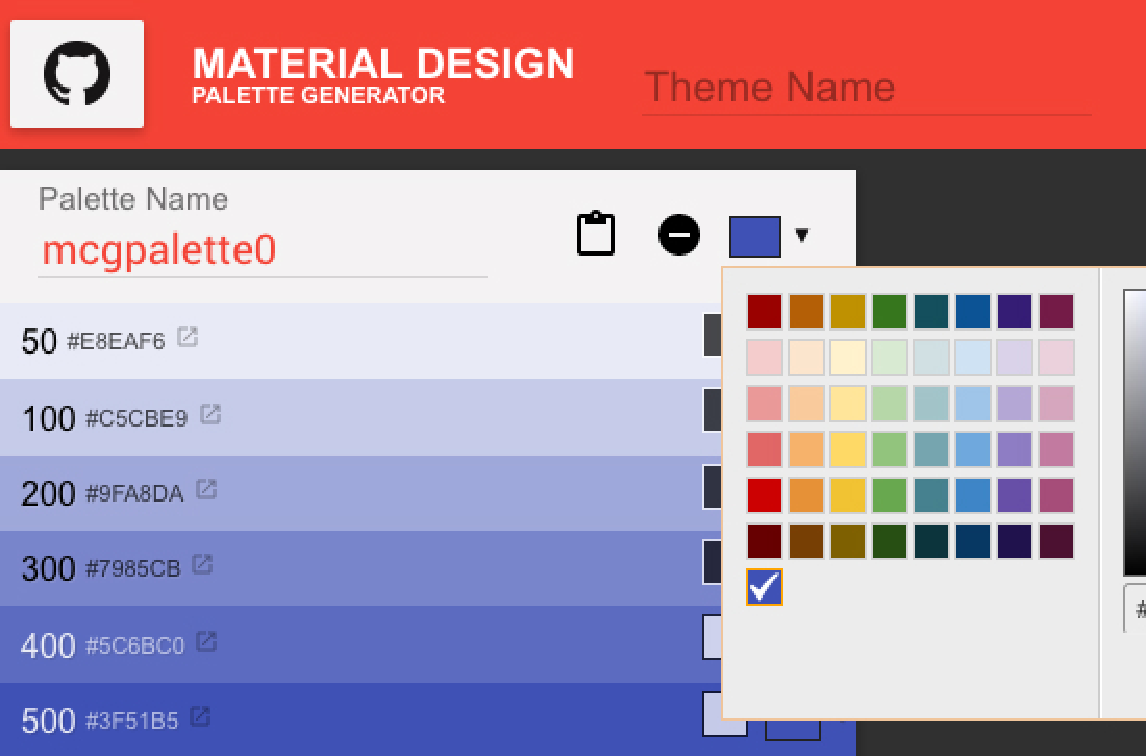
\includegraphics[width=414pt]{design-language-system/material-overrides/palette_generator_screenshot.pdf}

\subsection{Create a \_themes.scss file}
Being that we are creating our own themes, the cleanest thing for us to do would 
be to place it in it's own \_themes.scss file. In addition, assuming that the 
organization is going to build out more applications, giving it the ability to
plug and play the companies theme, will really speed up development for other
parts of the company. That being said, Razroo best practices is to create a lib
folder for styles.

\begin{forest}
  [libs
    [common
      [styles
        [\_themes.scss,file]
      ]
    ]
  ]
\end{forest}

and inside of it, we are going to create a \lstinline{_themes.scss} file. Our 
generated themes using our primary, or seconday colors might look something 
like this:

\begin{lstlisting}
$razroo-primary-blue: (
  50 : #e7f2f4,
  100 : #c3dee4,
  200 : #9cc8d3,
  300 : #74b2c1,
  400 : #56a2b3,
  500 : #3891a6,
  600 : #32899e,
  700 : #2b7e95,
  800 : #24748b,
  900 : #17627b,
  A100 : #b3eaff,
  A200 : #80dcff,
  A400 : #4dcfff,
  A700 : #33c8ff,
  contrast: (
    50 : #000000,
    100 : #000000,
    200 : #000000,
    300 : #000000,
    400 : #000000,
    500 : #ffffff,
    600 : #ffffff,
    700 : #ffffff,
    800 : #ffffff,
    900 : #ffffff,
    A100 : #000000,
    A200 : #000000,
    A400 : #000000,
    A700 : #000000,
  )
);
\end{lstlisting}

It's quite a bit, but I just wanted to visualize that all of this is created by
using the Material Design Palette Generator. 

\section{Using Libs \_themes.scss file }
Inside of our \lstinline{styles.scss} file, we can import our 
\lstinline{\_themes.scss} file. Assuming we are just changing the primary color
and secondary color, we can do the following: 
\begin{lstlisting}
@import '~@angular/material/theming';
@import 'libs/common/styles/_themes';  

//@include angular-material-theme($mat-light-theme-background);
$razroo-theme: mat-light-theme(mat-palette($razroo-primary-blue), mat-palette($razroo-secondary-red));
@include angular-material-theme($razroo-theme);
\end{lstlisting}

We now have our own custom themes that we have created. They are available 
globally to be used by other applications/teams. In addition, using the Angular 
mat-light-theme funciton(mat-dark-theme also an option), or app is now using
our exclusive theme. 

\section{Background + Foreground}
It is important to mention that per the Material Design guidelines, background
and foreground are not meant to represent brand. They are more so used to 
convey the energy of the application. For Razroo's Pixel Illustrator, we wanted
to create a very vibrant appliation. This meant that we wanted to use our own 
background and foreground colors. Doing something like this requires a bit more 
of effort probably from the Material team expecting you to do it less. There 
are three steps required to change the background to what you want. 

\begin{enumerate}
  \item Generate color theme maps, using our Material Design Palette Generator
  \item Create a backround theme, and foreground theme for our application.
  \item Create our own custom theme function.
  \item Creating a default background for html + body, being that this will 
  only work as an override for material design components. 
\end{enumerate}

\begin{lstlisting}[caption=Example of what a custom background theme looks like.]
// Background palette for light themes.
$razroo-theme-background: (
  status-bar: map_get($razroo-background-yellow, 300),
  app-bar:    map_get($razroo-background-yellow, 100),
  background: map_get($razroo-background-yellow, 50),
  hover:      rgba(map_get($razroo-background-yellow, 500), 0.04), // TODO(kara): check style with Material Design UX
  card:       map_get($razroo-background-yellow, 500),
  dialog:     map_get($razroo-background-yellow, 500),
  disabled-button: rgba(map_get($razroo-background-yellow, 500), 0.12),
  raised-button: map_get($razroo-background-yellow, 500),
  focused-button: $dark-focused,
  selected-button: map_get($razroo-background-yellow, 300),
  selected-disabled-button: map_get($razroo-background-yellow, 400),
  disabled-button-toggle: map_get($razroo-background-yellow, 200),
  unselected-chip: map_get($razroo-background-yellow, 300),
  disabled-list-option: map_get($razroo-background-yellow, 200),
);
\end{lstlisting}

\mybox{Your team should have a designer who figures out what the opposite color 
of your background is, in order to create foreground. However, you can use a tool 
such as such as Color Tool's 
\href{https://www.colortools.net/color_complementary.html}{Opposite Color Tool}}.
Then you can follow up with the Material Design Color Palette tool, and
create the appropriate color map.

\begin{lstlisting}[caption=What custom theme function would look like]
@function razroo-theme($primary, $accent, $warn: mat-palette($mat-red)) {
  @return (
    primary: $primary,
    accent: $accent,
    warn: $warn,
    is-dark: false,
    foreground: $mat-light-theme-foreground,
    background: $razroo-theme-background,
  );
}  
\end{lstlisting}

\begin{lstlisting}[caption=html and body override]
//@include angular-material-theme($mat-light-theme-background);
$razroo-theme: razroo-theme(mat-palette($razroo-primary-blue), mat-palette($razroo-secondary-red));

// Include the default theme styles.
@include angular-material-theme($razroo-theme);  
\end{lstlisting}

\section{Overriding Components}
After we have overridden our theme in general across the app, there will be 
times wherein we will need to override specific styles for the component. 
There really isn't any way to modify the styling ahead of time. The only way
is to target the specific material component's class, and to modify it when 
appropriate. However, what we can do, is consolidate all of our overridden
components in a singular place, so that it is well organized. For instance, 
let's say that we have a dialog that we would like to remove padding for 
in some scenarios, but keep it in others. We would put a dialog file inside of
our material overrides folder. Our folder/file structure will look like the
following: 

\begin{forest}
  [libs
    [common
      [styles
        [material-overrides
          [\_dialog.scss,file]
          [\_material-overrides.scss,file]
        ]
        [\_themes.scss,file]
      ]
    ]
  ]
\end{forest}


We import every material override into the main 
\lstinline{\_material-override.scss} file. Then, import the material-override 
file in our main \lstinline{styles.scss} file. 

\section{Overriding Overlay Components}
If you wish to override an overlay component, overlay components have a 
\lstinline{panelClass} property that can be used to target the overlay pane. 
For instance, with regards to dialogs, we have the ability to add a class doing
the following: 
\begin{lstlisting}
this.dialog.open(PxDialogComponent, {panelClass: 'razroo-no-padding-dialog'}) 
\end{lstlisting}

Now, we have the option to apply a css theme specifically to the 
razroo-no-padding-dialog class. 

\begin{lstlisting}
.myapp-no-padding-dialog .mat-dialog-container {
  padding: 0;
}
\end{lstlisting}

This gives us freedom moving forward, so that we can have multiple appearances
for our material components.

\section{Overriding Non Overlay Components}
Non overlay components, do not have the option to add a \lstinline{panelClass}.
The only solution which truly makes sense, is to create a global override on
the component itself. So, let's say that we wanted to change the appearance of
our material card components. Perhaps make the padding a little less pronounced.
We would do the following: 
\begin{lstlisting}[caption=\_mat-card.scss override]
  .mat-card {
    // this will be 8px
    padding: rz-space-multiplier(1);
  }
\end{lstlisting}

\section{Wrapping up}
Material is, and will for a very long time, be the premier design language for
Angular. It is incredibly simple to set up, and a breeze to modify. In my humble 
opinion, it is one of the three greatest architectural decisions someone can make 
for Angular(State management, and extensive unit testing being the others).
